\chapter{Теоретическая часть}

\section{Основные определения и понятия}
Для решения поставленной задачи (см. раздел \ref{задание}) необходимо быть ознакомленным с математическими объектами, методами и понятиями, описанными далее.
\subsection{Конечно-элементная сетка с заданным векторным полем}
Метод конечных элементов представляет собой наиболее распространенный приближенный метод в механике твердого тела. Основа МКЭ – это разбиение математической модели конструкции на некоторое количество непересекающихся подобластей простой геометрии с конечным размером. Эти подобласти называются конечными элементами или просто элементами, а разбиение дискретизацией.

Форма конечных элементов будет зависеть от типа рассчитываемой конструкции и характера ее деформаций. Например, конечными элементами в расчете стержневых конструкций (балок, колонн, рам, ферм) будут участки стержней, при расчетах двумерных континуальных систем (пластин, плит или оболочек) – прямоугольные или треугольные подобласти, а при расчете трехмерных конструкций (массивов или толстых плит) – подобласти в виде тетраэдров или параллелепипедов. Множество элементов, на которые разбита конструкция, называется конечно-элементной сеткой. Но в отличие от настоящей конструкции в дискретной модели связывание конечных элементов происходит только в определенных точках (узлах) некоторым известным количеством узловых параметров. \cite{chislaki}

\begin{figure}[H]
	\hfill
	\begin{subfigure}{.4\textwidth}
		\centering
		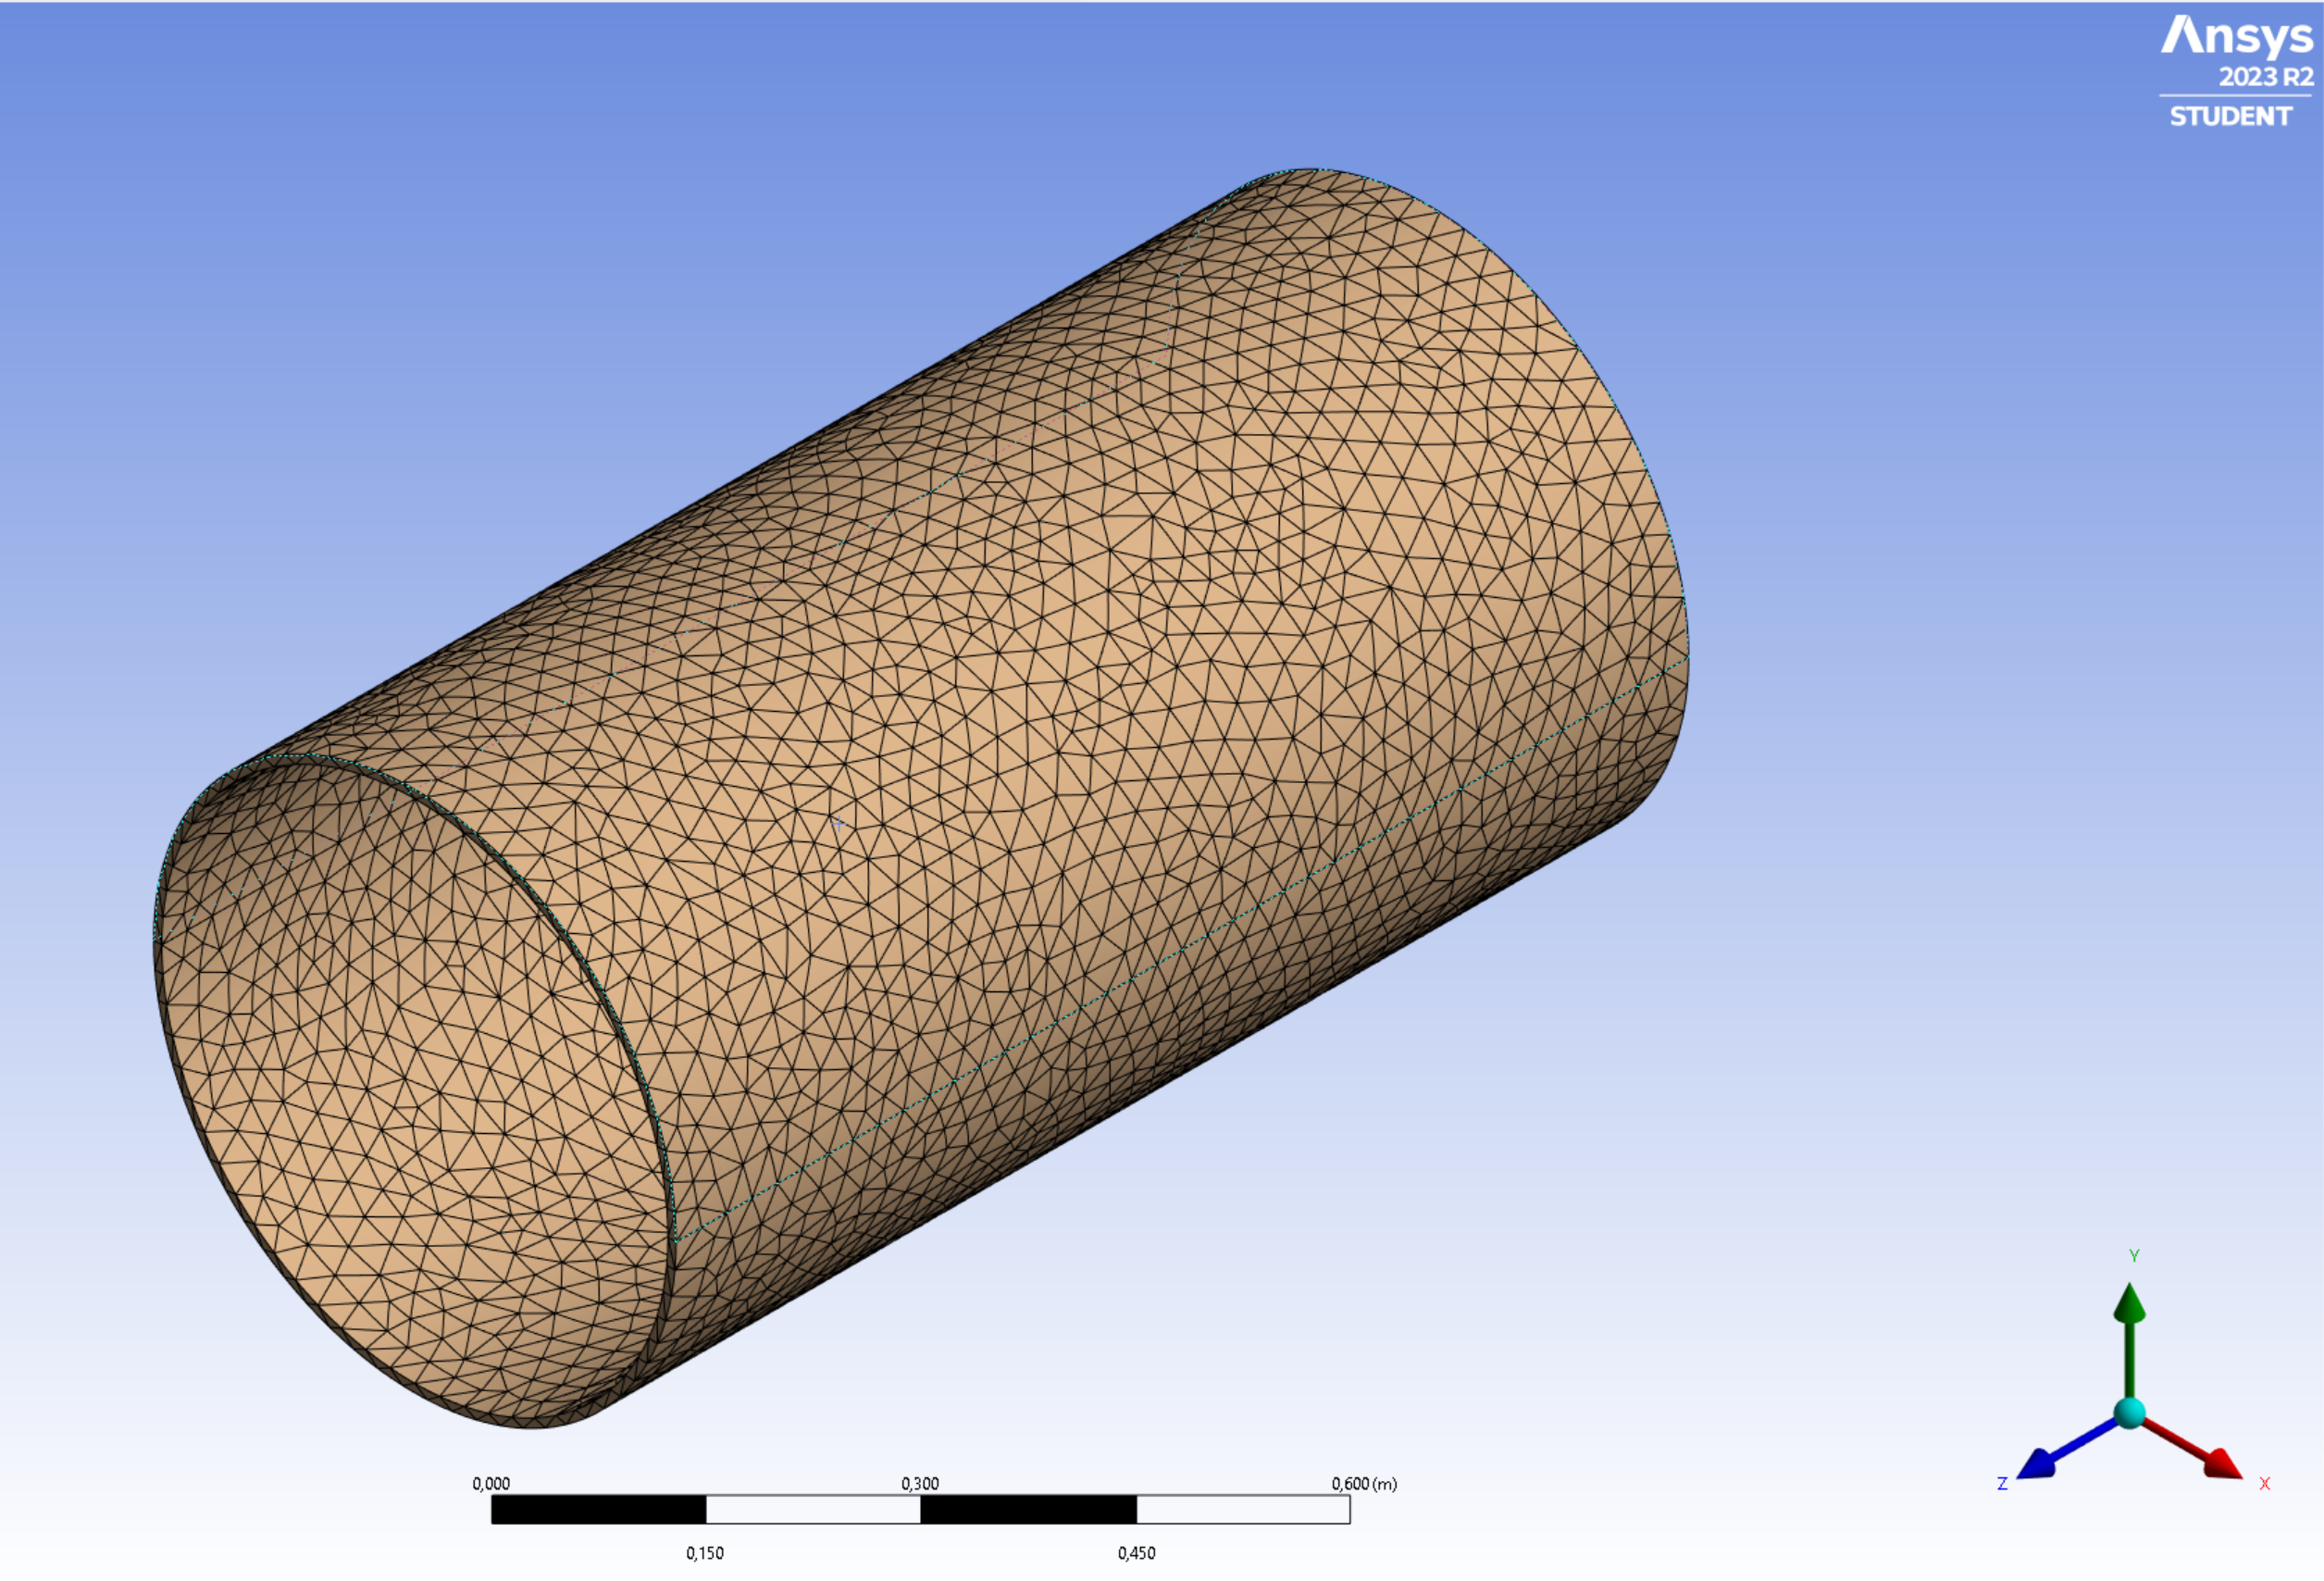
\includegraphics[width=\linewidth]{img/setka_example}
		\caption{Трехмерная конечно-элементная сетка, построенная для геометрии цилиндра}
	\end{subfigure}
	\hfill
	\begin{subfigure}{.5\textwidth}
		\centering
		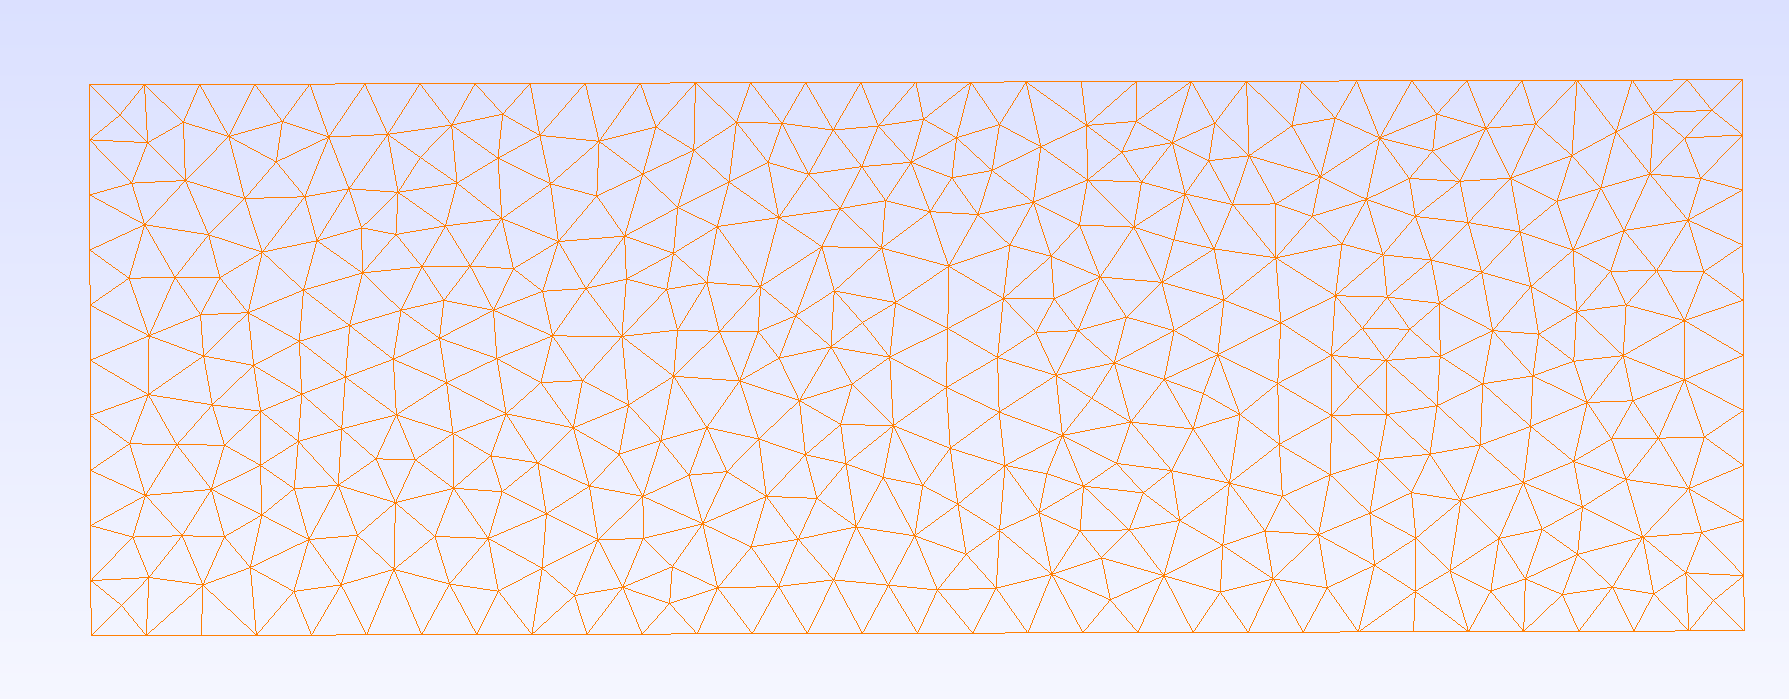
\includegraphics[width=\linewidth]{img/setka_example_2d}
		\caption{Двухмерная конечно-элементная сетка, построенная по модели прямоугольника}
		\label{2d_setka}
	\end{subfigure}
	\hfill
	\caption{Примеры конечно-элементных сеток}
\end{figure}

Также на сетке можно дополнительно задать или рассчитать некоторые данные о рассматриваемой модели. Например векторное поле, представляющее вектор скорости среды (см. Рисунок \ref{setka_with_vector_field}).

\begin{figure}[H]
	\centering
	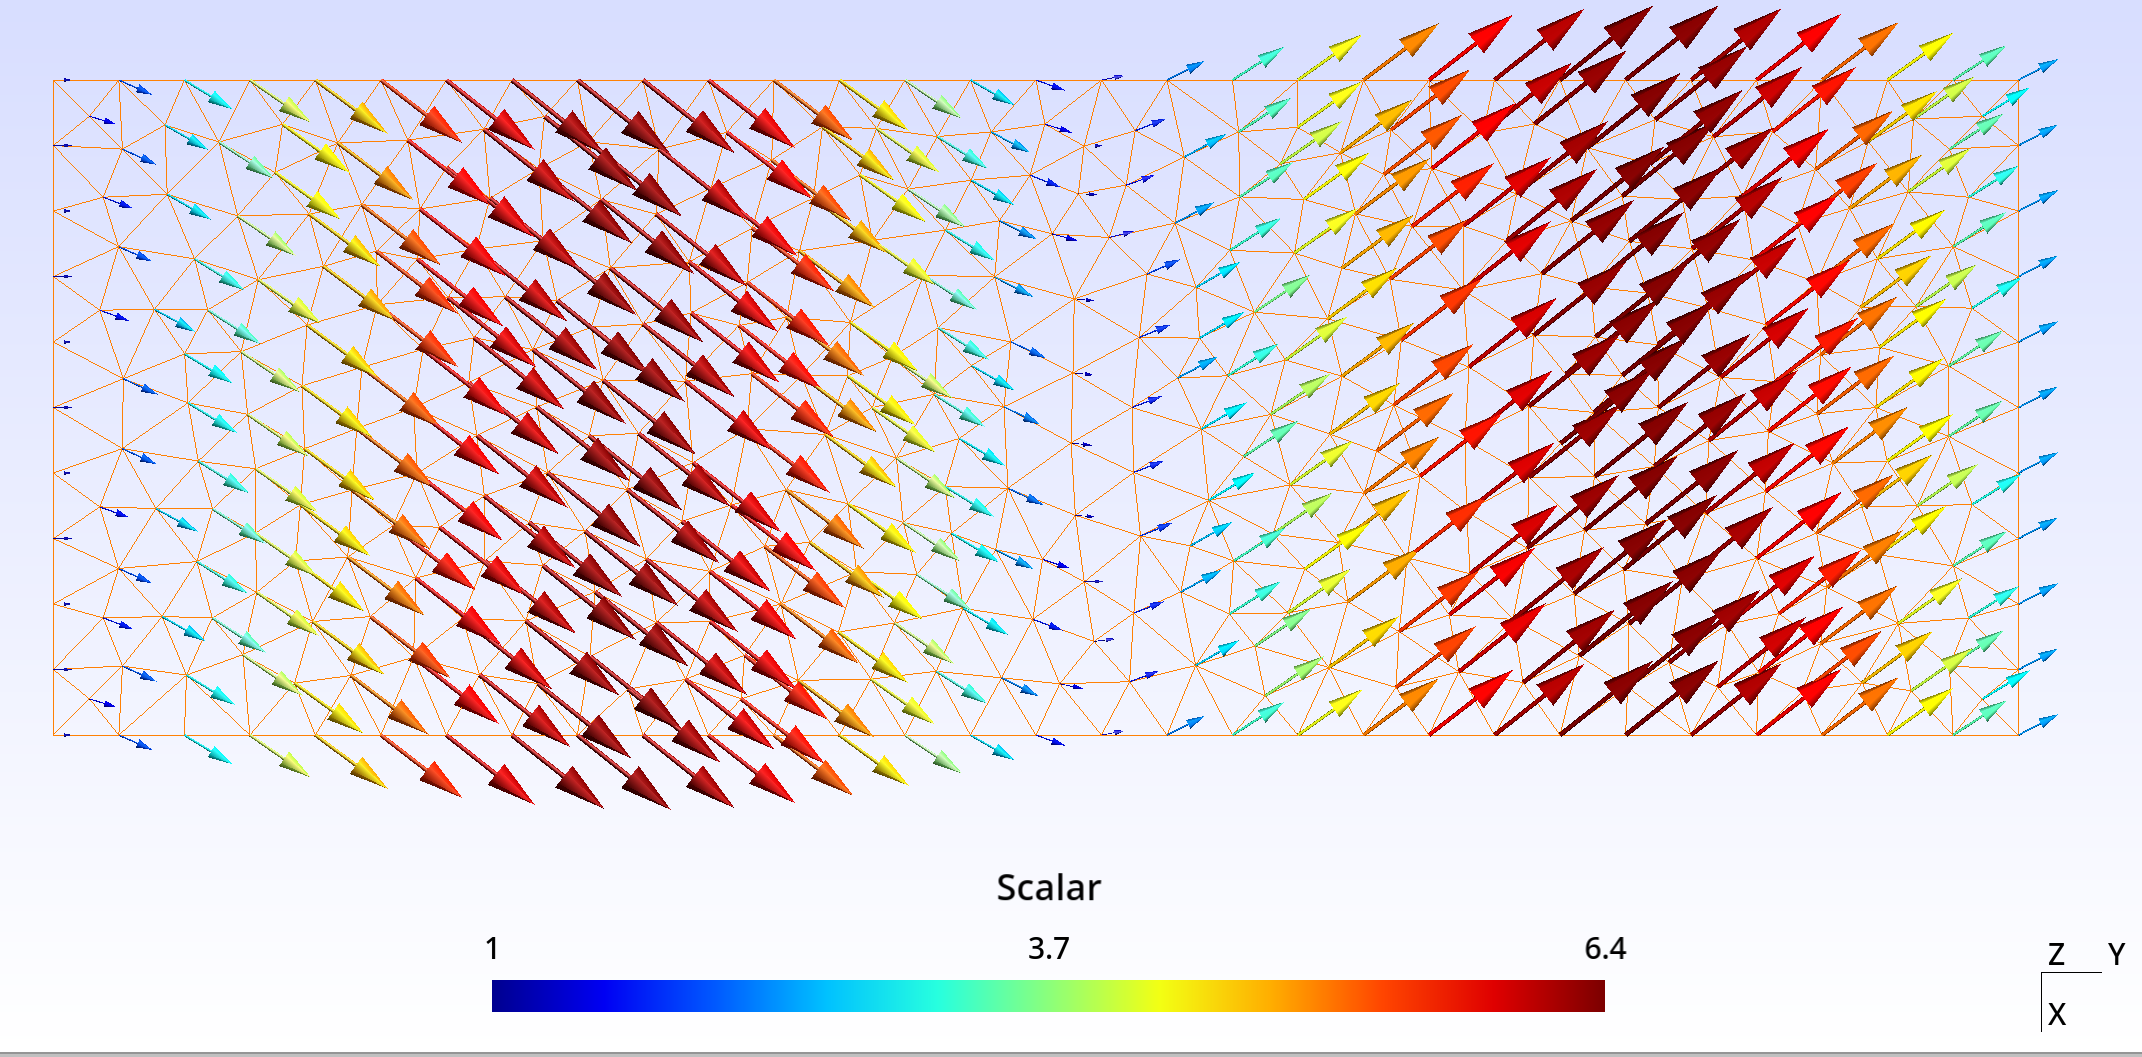
\includegraphics[width=\linewidth]{img/setka_with_vector_field}
	\caption{Визуализация векторного поля на сетке с Рисунка \ref{2d_setka}}
	\label{setka_with_vector_field}
\end{figure}

\subsection{Линии тока}
Для наглядного представления векторных полей применяют линии тока (далее ЛТ). Например, в магнитной динамике ЛТ называют силовыми линиями. ЛТ, проходящей через точку $M$ называют такую кривую, которая в каждой своей точке имеет касательную, параллельную вектору скорости в данной точке в данный момент времени. ЛТ будут отображать направление векторного поля (Рисунок \ref{cur_lines}).

\begin{figure}[H]
	\centering
	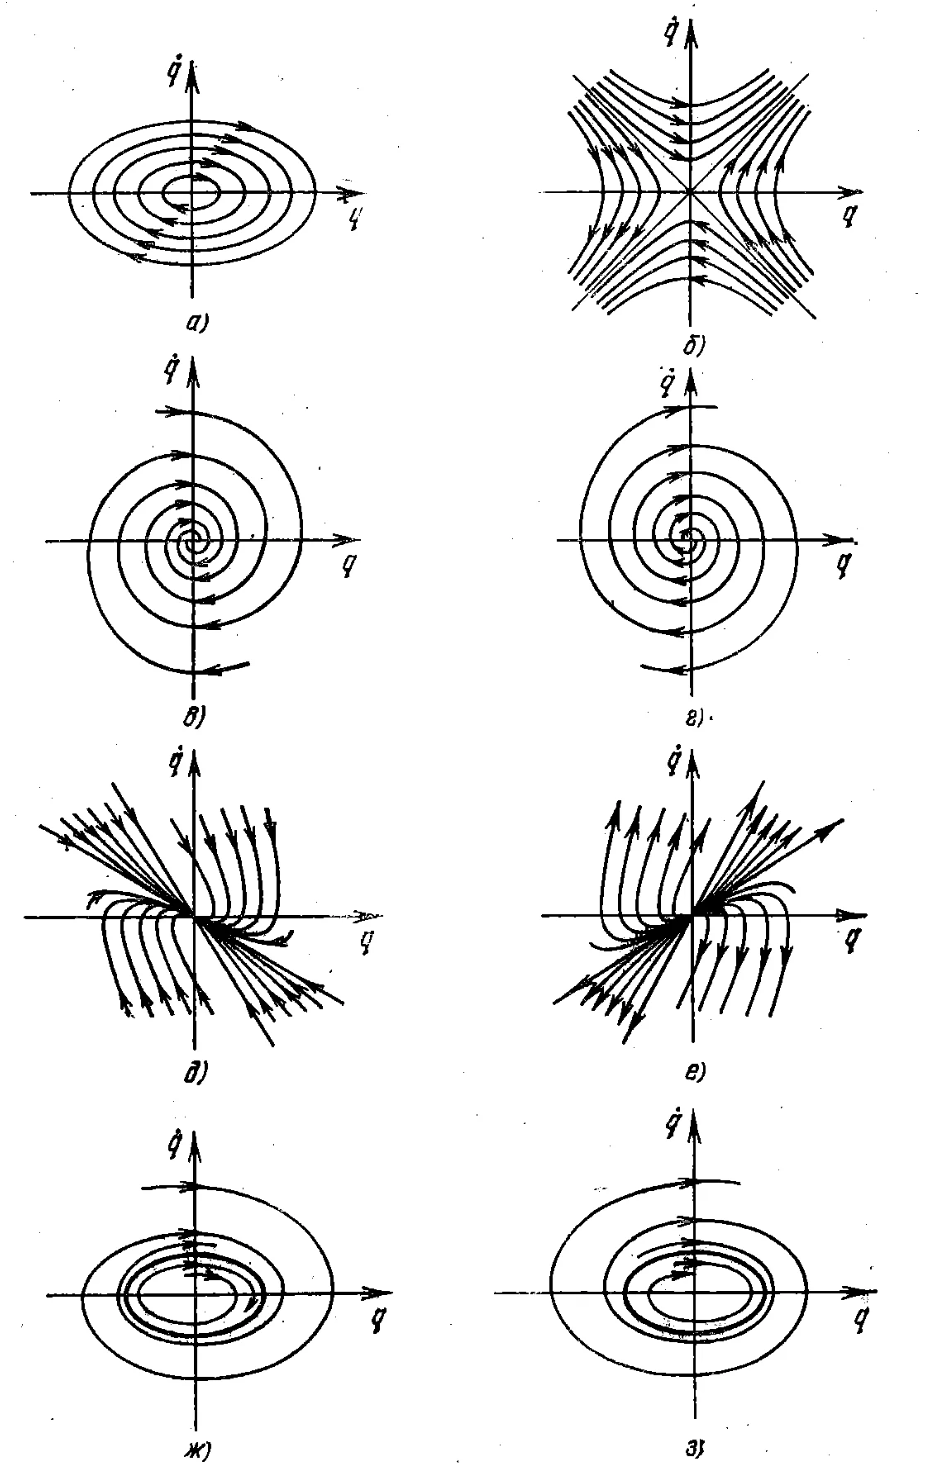
\includegraphics[width=.5\linewidth]{img/cur_lines}
	\caption{Примеры линий тока}
	\label{cur_lines}
\end{figure}

\subsection{Базовая точка}
Алгоритм построения ЛТ начинается с инициализации базовой точки в пределах заданной расчетной сетки. Базовая точка является начальной точкой при построении линия тока. Каждая базовая точка определяет одну линию тока. Для работы алгоритма необходимо будет работать с КЭ, в котором находится текущая точка. Для нахождения такого КЭ далее будут рассмотрены несколько алгоритмов.

\subsection{Интерполяция на сетке}
Интерполяция --- это поиск значений функции в промежуточных точках по известным значениям функции в окружающих точках.
\begin{align*}
	y_i = f(x_i),\quad i=\overline{1\dots n}\\
	y_i = F(x_i),\quad i=\overline{1\dots n}
\end{align*}
То есть для функции $f_i$, значения которой известны лишь в точках $x_i$, необходимо найти интерполирующую её функцию $F$, которая определена во всех промежуточных точках, а в точках $x_i$ её значение совпадает с исходной функцией.

Вид сетки определяет, какой метод интерполяции может быть к ней применен.
\section{Постановка задачи}
При заданной базовой точке $M$ на конечно-элементной сетке, состоящий из набора конечных элементов $\left\{E_i\right\}$, построить из этой базовой точки линию тока. Конечно-элементная сетка может быть разных видов: треугольная, четырехугольная. Каждому КЭ $E_i$ соответствует набор его вершин $v_{ij}$. Для каждой вершины задано некоторое значение векторного поля $\vec{f}\left(v_{ij}\right)$.
\begin{equation*}
	\vec{f}: v_{ij} \to \mathbb{R}^3,
\end{equation*}
\gde{
{$j$}{обозначает количество вершин КЭ и задается типом сетки}
}
Например, треугольные и четырехугольные сетки будут иметь значения $j=3$ и $j=4$ соответственно.

\section{Метод построения линий тока}\label{method}
Обозначим размер шага для построения линии тока по осям $x, y$ соотвественно за $dx, dy$. Высчитывать их будем исходя из размеров сетки
\begin{align*}
	dx &= \frac{\max\limits_{i,\, j}\left({v_{ij}}_x\right)-\min\limits_{i,\, j}\left({v_{ij}}_x\right)}{k},\\ 
	dy &= \frac{\max\limits_{i,\, j}\left({v_{ij}}_y\right)-\min\limits_{i,\, j}\left({v_{ij}}_y\right)}{k},\\ 
	dz &= \frac{\max\limits_{i,\, j}\left({v_{ij}}_z\right)-\min\limits_{i,\, j}\left({v_{ij}}_z\right)}{k},
\end{align*}
\gde{
{$k$}{желаемая точность построения линии тока, например $k=1000$}
}
Обозначим базовую точку $M$ за первую текущую точку $C_0$ и сохраним её в список точек, из которых состоит линия тока. Линию тока будем обозначать как $L$.
\begin{equation*}
	C_0 = M,\quad L=(C_0)
\end{equation*}
Итерация метода построения ЛТ состоит из следующих шагов:
\begin{enumerate}
	\item Определить, находится ли текущая точка в том же КЭ, который был рассмотрен в прошлой итерации. Для этого воспользуемся функцией индикатором
	\begin{equation*}
		I(C_i\in E_{i-1}).
	\end{equation*}
	Если $C_i\in E_{i-1}$ то пропускаем шаг \ref{find_E}, то есть $E_i=E_{i-1}$.
	Заметим, что на первой итерации алгоритма мы точно знаем, что $C_i\notin E_{i-1}$, ведь $E_{i-1}$ ещё ни разу не был определён.
	\item\label{find_E} Определить текущий КЭ -- тот КЭ, в котором находится текущая точка. Обозначим некую функцию, которая определяет текущий КЭ за $E$, она является отображением из множества всех точек пространства на пространство КЭ. Также учтём крайний случай, когда текущая точка находится за пределами модели, тогда функция будет отображать точку в $\varnothing$
	\begin{equation*}
		E: \mathbb{R}^3 \to \left\{E_i\right\} \cup \varnothing
	\end{equation*}
	Тогда текущий элемент на i-ой итерации $E_i$ будет выражаться как функция $E(C_{i-1})$;
	\item Если $E_i=\varnothing$, то остановка;
	\item Определить величину векторного поля $\vec V$ в текущей точке, интерполируя между величинами векторного поля в вершинах текущего КЭ. Обозначим функцию, которая проводит данную интерполяцию за $A$. Функция $A$ отображает $j$ вершин конечного элемента с значениями векторного поля в них в один вектор в текущей точке. Получим величину векторного поля:
	\begin{equation*}
		A(v_{i1},v_{i2},\dots,v_{ij}, \vec{f}(v_{i1}),\vec{f}(v_{i2}),\dots,\vec{f}(v_{ij}), C_i) = \vec{A}_{i}\in\mathbb{R}^3;
	\end{equation*}
	\item Получить координаты следующей точки линии тока. Для этого нормируем величину векторного поля в текущей точке и прибавим к её координатам с коэффициентами $dx, dy$. Тогда координаты новой точки линии тока выражаются следующим образом
	\begin{equation*}
		\begin{cases}
		{C_i}_x &= {C_{i-1}}_x + dx\cdot\left(\frac{\vec{A}_i}{|\vec{A}_i|}\right)_x,\\
		{C_i}_y &= {C_{i-1}}_y + dy\cdot\left(\frac{\vec{A}_i}{|\vec{A}_i|}\right)_y,\\
		{C_i}_z &= {C_{i-1}}_z + dz\cdot\left(\frac{\vec{A}_i}{|\vec{A}_i|}\right)_z;
		\end{cases}
	\end{equation*}
	\item Занести новую точку линии тока в список $L$
\end{enumerate}

Подведём итоги. Функции, которые необходимо реализовать:
\begin{itemize}
	\item $E$ --- определение текущего элемента по текущей точке;
	\item $I$ --- индикатор, проверка нахождения точки в заданном КЭ;
	\item $A$ --- интерполяция значений векторного поля в вершинах КЭ для текущей точки.
\end{itemize}
